\chapter{Resumen de los Resultados}\label{Chap:Results}
\markboth{\MakeUppercase{Resumen de los Resultados}}{}

En este capítulo se presenta un resumen de los principales resultados obtenidos durante esta investigación.
Primero se presenta un esquema de anotación diseñado para capturar las entidades y relaciones semánticas fundamentales en un texto, independiente del idioma y dominio (Sección~\ref{results:schema}.
Basado en este esquema de anotación se presentan tres corpus anotados manualmente, en documentos en idioma español del dominio de la salud~(Sección~\ref{results:corpus}).
A partir de estos recursos se diseña una tarea computacional que consiste en la detección automática de entidades y relaciones, con métricas y escenarios de evaluación que permiten una comparación objetiva entre diferentes sistemas~(Sección~\ref{results:tasks}).
Con vistas a automatizar el proceso de evaluación de soluciones a esta tarea computacional, se propone una infraestructura que brinda implementaciones base~(\textit{baseline}) de algoritmos y todas las herramientas necesarias para desarrollar y evaluar implementaciones más complejas~(Sección~\ref{results:infrastructure}).
Se presenta además la evaluación de un conjunto de sistemas propuestos por múltiples equipos de investigadores en 3 ediciones del evento \textit{eHealth Knowledge Discovery Challenge}~(Sección~\ref{results:challenge}), que han sido evaluados respectivamente en las 3 versiones de los corpus anotados en esta investigación.
Finalmente, a partir de la experiencia acumulada en la construcción de recursos lingüísticos, se diseña un entorno de anotación asistida basada en aprendizaje automático activo~(Sección~\ref{results:assisted-ann}).
A modo de resumen, la Figura~\ref{fig:conceptualmap} presenta un esquema conceptual del ecosistema computacional diseñado en esta Tesis.

\begin{figure}
    \centering
    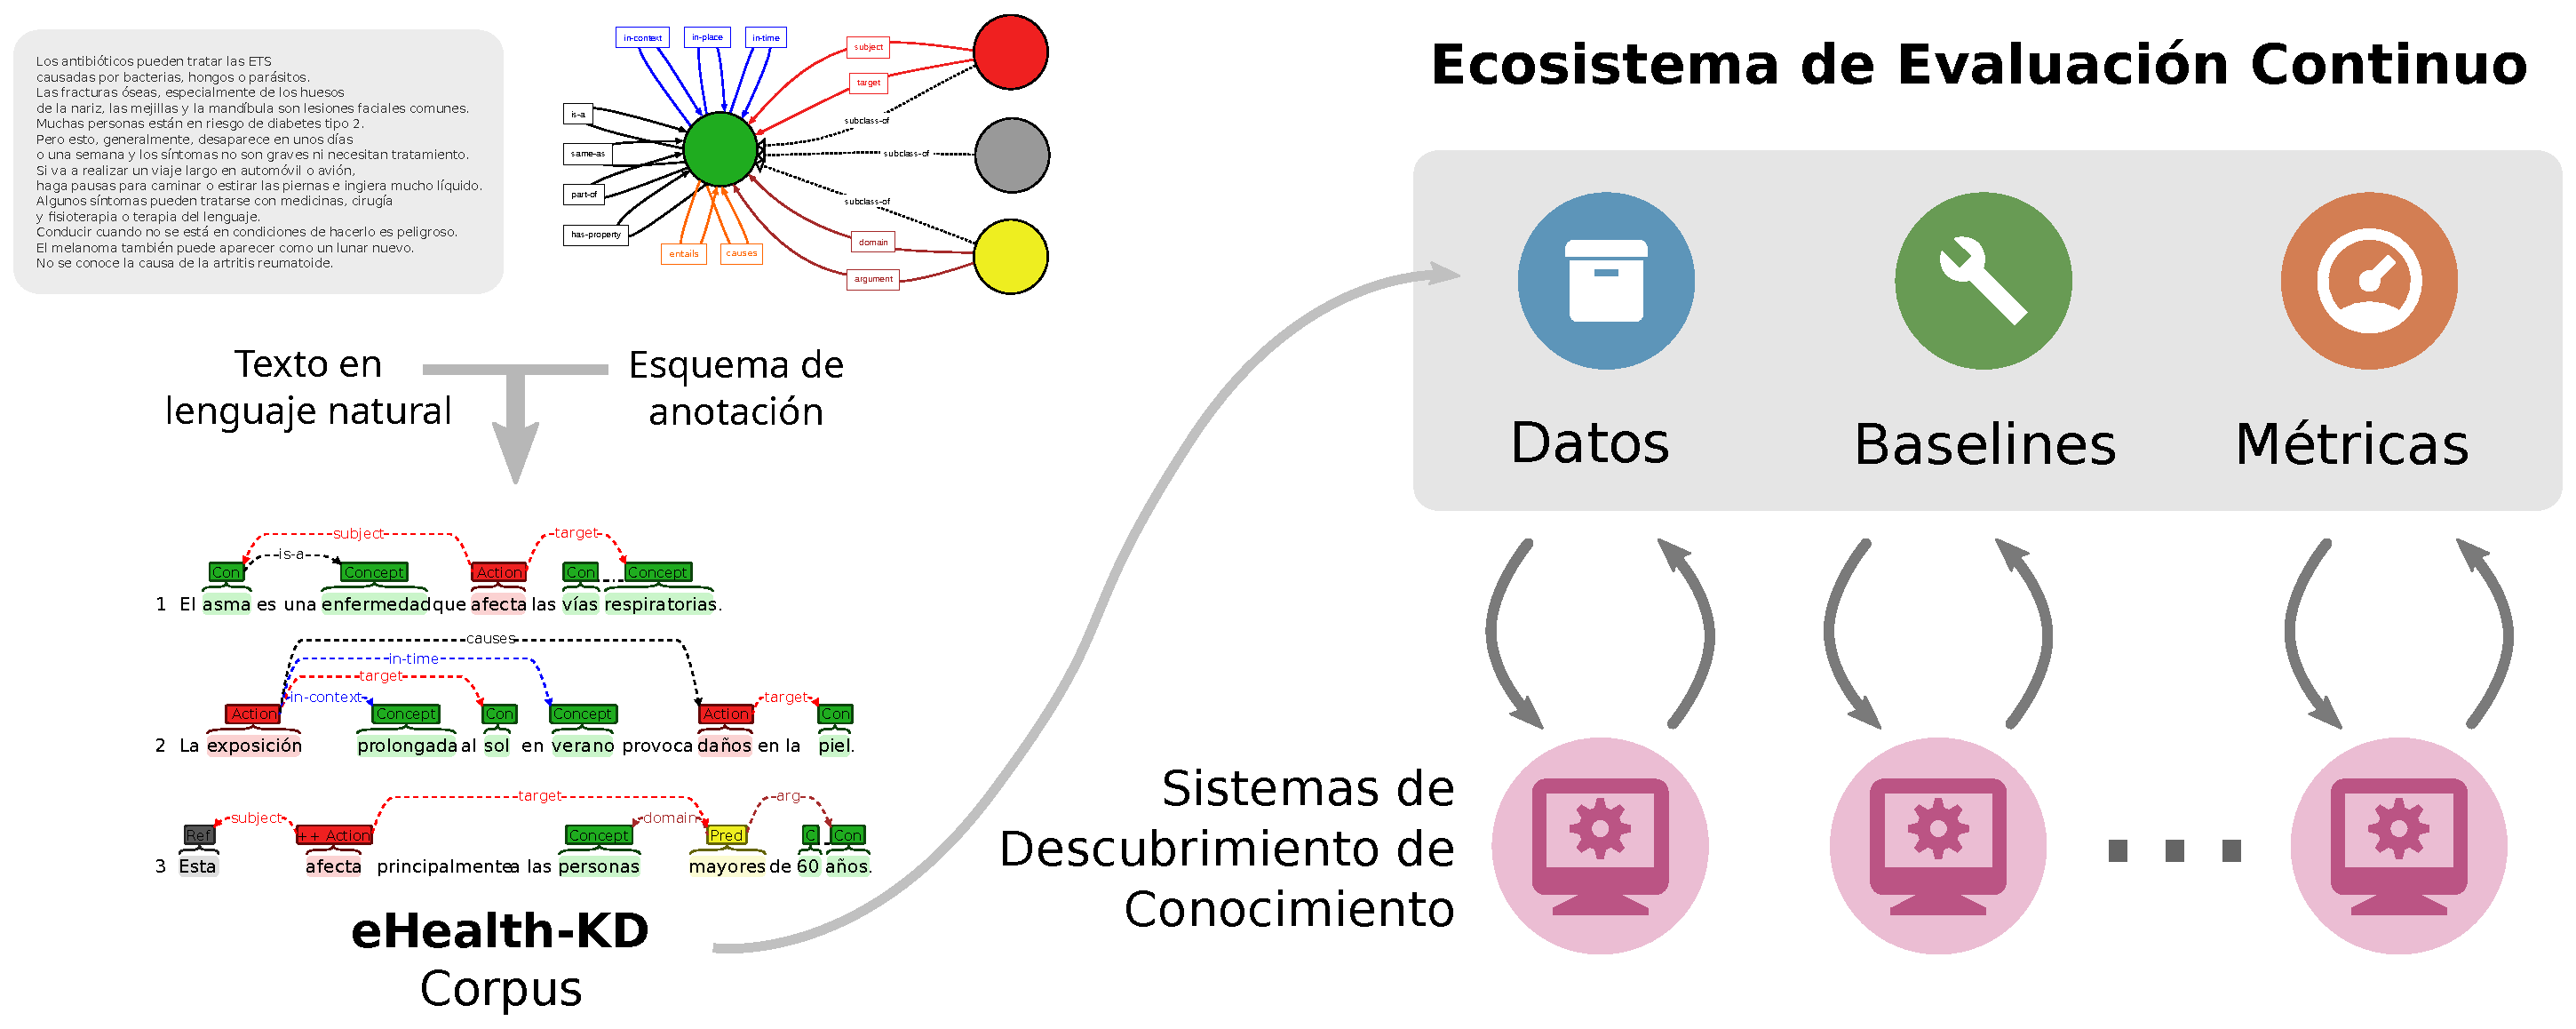
\includegraphics[width=\textwidth]{Images/Chapters/graphical-abstract.pdf}
    \caption{Esquema conceptual del ecosistema computacional diseñado en esta tesis.}
    \label{fig:conceptualmap}
\end{figure}

\section{Esquema de anotación}\label{results:schema}

El proceso de descubrimiento de conocimiento en lenguaje natural comienza por la identificación en el texto de los conceptos y relaciones más relevantes en un dominio. Para ello es necesario definir un modelo de representación semántico que capture estos conceptos. Dicho modelo se concreta en un esquema de anotación que permite a expertos humanos construir un corpus anotado semánticamente. Construir sistemas de descubrimiento de conocimiento automáticos generalizables a cualquier dominio requiere que los conceptos y relaciones representados sean de propósito general. Además, el esquema de anotación debe lograr un balance adecuado entre su capacidad expresiva y su simplicidad para ser anotado por expertos humanos y algoritmos de aprendizaje automático.

En esta Tesis se propone un esquema de anotación con estas características, que se inspira en varios recursos.
En términos de representación del conocimiento, se basa en dos modelos diferentes para la conceptualización de la realidad: ontologías y teleologías.
La Figura~\ref{fig:example} muestra una anotación de ejemplo de tres oraciones con diferentes grados de complejidad.
El esquema de anotación se explica en profundidad en el Capítulo~\ref{Chap:Schema}.

\begin{figure}[htb]
    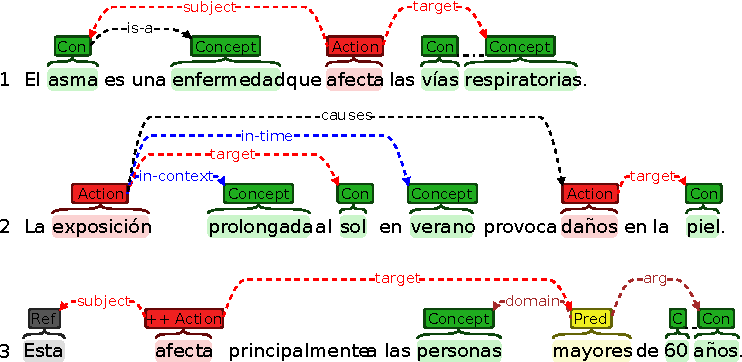
\includegraphics[width=\textwidth]{Images/Chapters/ExampleSentences.pdf}
    \caption[Ejemplos de anotación.]{Ejemplo de anotación de tres oraciones. La anotación muestra las entidades y relaciones más relevantes definidas en el esquema de anotación propuesto.}
    \label{fig:example}
\end{figure}

La parte ontológica del esquema proporciona una representación de entidades en términos de sus relaciones jerárquicas y estructurales~(es decir, \texttt{is-a}, \texttt{part-of}, \texttt{has-property} y \texttt{same-as}).
Estas relaciones se basan en el diseño de ontologías de propósito general como ConceptNet~\cite{speer2017conceptnet} y YAGO~\cite{suchanek2007yago}.
La parte teleológica del esquema proporciona una representación de eventos o procesos que transforman entidades, es decir, representan las interacciones entre las entidades.
Esto está respaldado por una estructura basada en el trabajo de~\citet{teleologies}.
El significado semántico exacto de estos conceptos y relaciones se explica con más detalle a continuación.

El elemento más importante de la anotación es la estructura Sujeto-Acción-Objetivo~(\textit{Subject-Action-Target}), que captura la interacción principal entre entidades en oraciones factuales.
En esta interacción participan dos tipos de entidades fundamentales: \texttt{Concept} y \texttt{Action}.
Un \texttt{Concept} define una entidad relevante en el dominio, que puede ser una sola palabra o múltiples tokens, contiguos o no.
Una \texttt{Action} representa un proceso o evento causado por uno o más \texttt{Concept}~(mediante la relación \texttt{subject}) y que impacta en uno o más \texttt{Concepts}~(mediante la relación \texttt{target}).
Las entidades conectadas a los roles \texttt{subject} y \texttt{target} también pueden ser de tipo \texttt{Action}, lo que permite que los conceptos simples se compongan en otros más complejos.
La estructura Sujeto-Acción-Objetivo definida en este esquema se basa en una versión simplificada del marco teleológico propuesto por~\citet{teleologies}. Los elementos \textit{Object} y \textit{Action} en las teleologías están representados en este esquema por \texttt{Concept} y \texttt {Action} respectivamente.
El rol \textit{Function} en las teleologías, que expresa una instancia de un objeto que realiza una acción, puede equipararse aproximadamente al uso de una entidad de tipo \texttt{Action} ocupando el rol \texttt{subject} o \texttt{target} de otras acciones.

Una adición importante a este esquema de anotación es la entidad \texttt{Predicate}.
Los predicados modelan la existencia de conceptos complejos~(mediante el rol \texttt{domain}) que dependen de algunas condiciones previas~(mediante el rol \texttt{arg}).
Por ejemplo, en la Figura~\ref{fig:example}, Oración 3, el concepto de \textit{personas mayores de 60 años} se puede definir con una anotación detallada, considerando ``\textit{personas}'' como el dominio y ``\textit{60 años}'' como argumento. Esta anotación permite la captura de información más detallada en lugar de simplemente anotar la frase completa como un concepto de varias palabras.
Otra adición es \texttt{Reference}, que representa conceptos mencionados de forma implícita en una oración.
Las palabras más comunes etiquetadas como referencias son: ``\textit{esto}'', ``\textit{el}'', ``\textit{la}'', ``\textit{este}'', es decir , generalmente pronombres y artículos.

Para refinar aún más la interpretación semántica de cada entidad, se define un conjunto de 4 atributos:
\texttt{uncertain}, \texttt{emphasized}, \texttt{diminished} y \texttt{negated}.
Estos atributos a menudo se pueden identificar mediante adjetivos u otros patrones sintácticos que aparecen en el contexto de una entidad determinada, pero en lugar de anotar toda la frase, la entidad correspondiente se etiqueta con el atributo.
Por ejemplo, en la oración 3 de la Figura~\ref{fig:example}, la acción ``\textit{afecta}'' se etiqueta con \texttt{emphasized}, debido a la presencia de la palabra ``\textit{principalmente}'', y se representa en la anotación con un signo \texttt{++} en la entidad.
El uso de atributos permite la captura de conceptos semánticos más refinados~(es decir, grados de énfasis, negación, incertidumbre) mientras se mantiene el agnosticismo del idioma, ya que es irrelevante en qué parte del texto se presenta esa información.
Puede aparecer explícitamente en una sola palabra~(por ejemplo, un adjetivo) o implícitamente mediante frases idiomáticas u otros patrones lingüísticos sutiles.
Estos atributos aumentan el rango semántico del esquema de anotación sin aumentar el número de tokens que deben ser anotados.

Este esquema define 4 relaciones ontológicas principales: \texttt{is-a}, \texttt{same-as}, \texttt{part-of} y \texttt{has-property}, con su semántica habitual, que pueden vincular cualquier par de entidades, simples o compuestas, entre sí.
Estas relaciones permiten la representación del conocimiento estructural, por ejemplo, conceptos relacionados en una estructura jerárquica y conceptos que son componentes de otros conceptos.
Se define dos relaciones adicionales, \texttt{causes} y \texttt{entails}, para capturar causalidad e implicación lógica respectivamente.
Estas relaciones, respectivamente de naturaleza teleológica y ontológica, son de gran importancia porque permiten la construcción de sistemas de razonamiento que pueden llegar a conclusiones y producir nuevos conocimientos a partir de un corpus existente.

Además, se definen 3 relaciones contextuales, para recopilar conocimientos importantes que generalmente aparecen como complementos gramaticales: \texttt{in-time}, \texttt{in-place}, \texttt{in-context}.
La relación \texttt{in-time} se usa para expresar la duración de un evento.
La relación \texttt{in-place} se usa para identificar una ubicación específica para una entidad de tipo \texttt{Action} o \texttt{Concept}.
La relación \texttt{in-context} es una relación más genérica que representa una dependencia general entre dos entidades cuya naturaleza exacta no puede definirse por ninguna de las otras relaciones.
Estas relaciones también son de naturaleza teleológica, ya que no definen una afirmación en sí, sino que son útiles para especificar las condiciones en las que ocurren algunos eventos.
Por ejemplo, en la Oración 2~(Figura~\ref{fig:example}, la anotación \textit{exposición}~$\Rightarrow$~\texttt{in-context}~$\Rightarrow$~\textit {prolongado} no implica que el concepto ``\textit{exposición}'' incondicionalmente tenga la calidad ``\textit{prolongado}''. Solo cuando este concepto complejo se usa como \texttt{subject} o \texttt{target} de una entidad de tipo \texttt{Action} o en otra relación, es que la contextualización adquiere un significado.

La figura~\ref{fig:model} resume el esquema de anotación. Este esquema está diseñado para capturar el conocimiento semántico más relevante presente en un corpus arbitrario.
Por esta razón, no se definieron relaciones o entidades específicas de dominio~(es decir, no hay entidades específicas para enfermedades, pacientes, tratamiento, etc.).
Por el contrario, las relaciones específicas de dominio pueden representarse mediante acciones y sus roles correspondientes.

\begin{figure}[htb]
    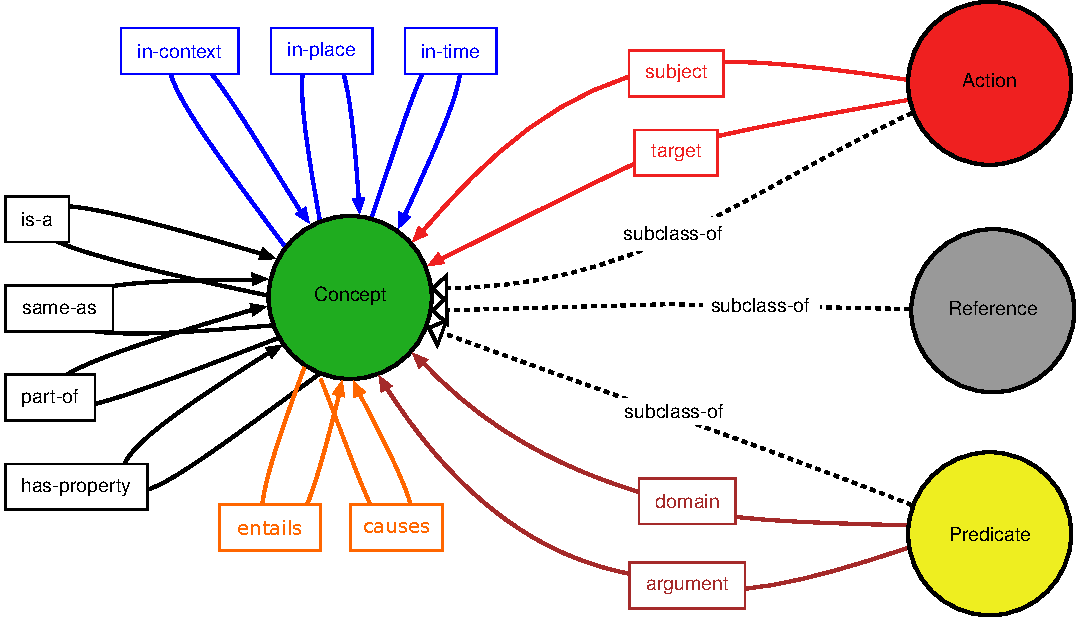
\includegraphics[width=\textwidth]{Images/Chapters/AnnotationModelDiagram.pdf}
    \caption{Diagrama resumen del esquema de anotación general.}
    \label{fig:model}
\end{figure}

\section{Corpus}\label{results:corpus}

Basado en el esquema de anotación definido en la Sección~\ref{results:schema} se anotaron un total de 3 corpus en idioma español.
Cada corpus corresponde a una edición de la campaña de anotación \textit{eHealth-KD} que se presenta en la Sección~\ref{results:challenge}. El primer corpus se anotó con una variante ligeramente diferente del esquema de anotación, debido a que este esquema fue evolucionando durante el proceso de investigación.
En esta Sección se presentan las características fundamentales de estos corpus, incluyendo la estrategia
de anotación seguida en cada caso.

\begin{figure}[htb]
    \centering
    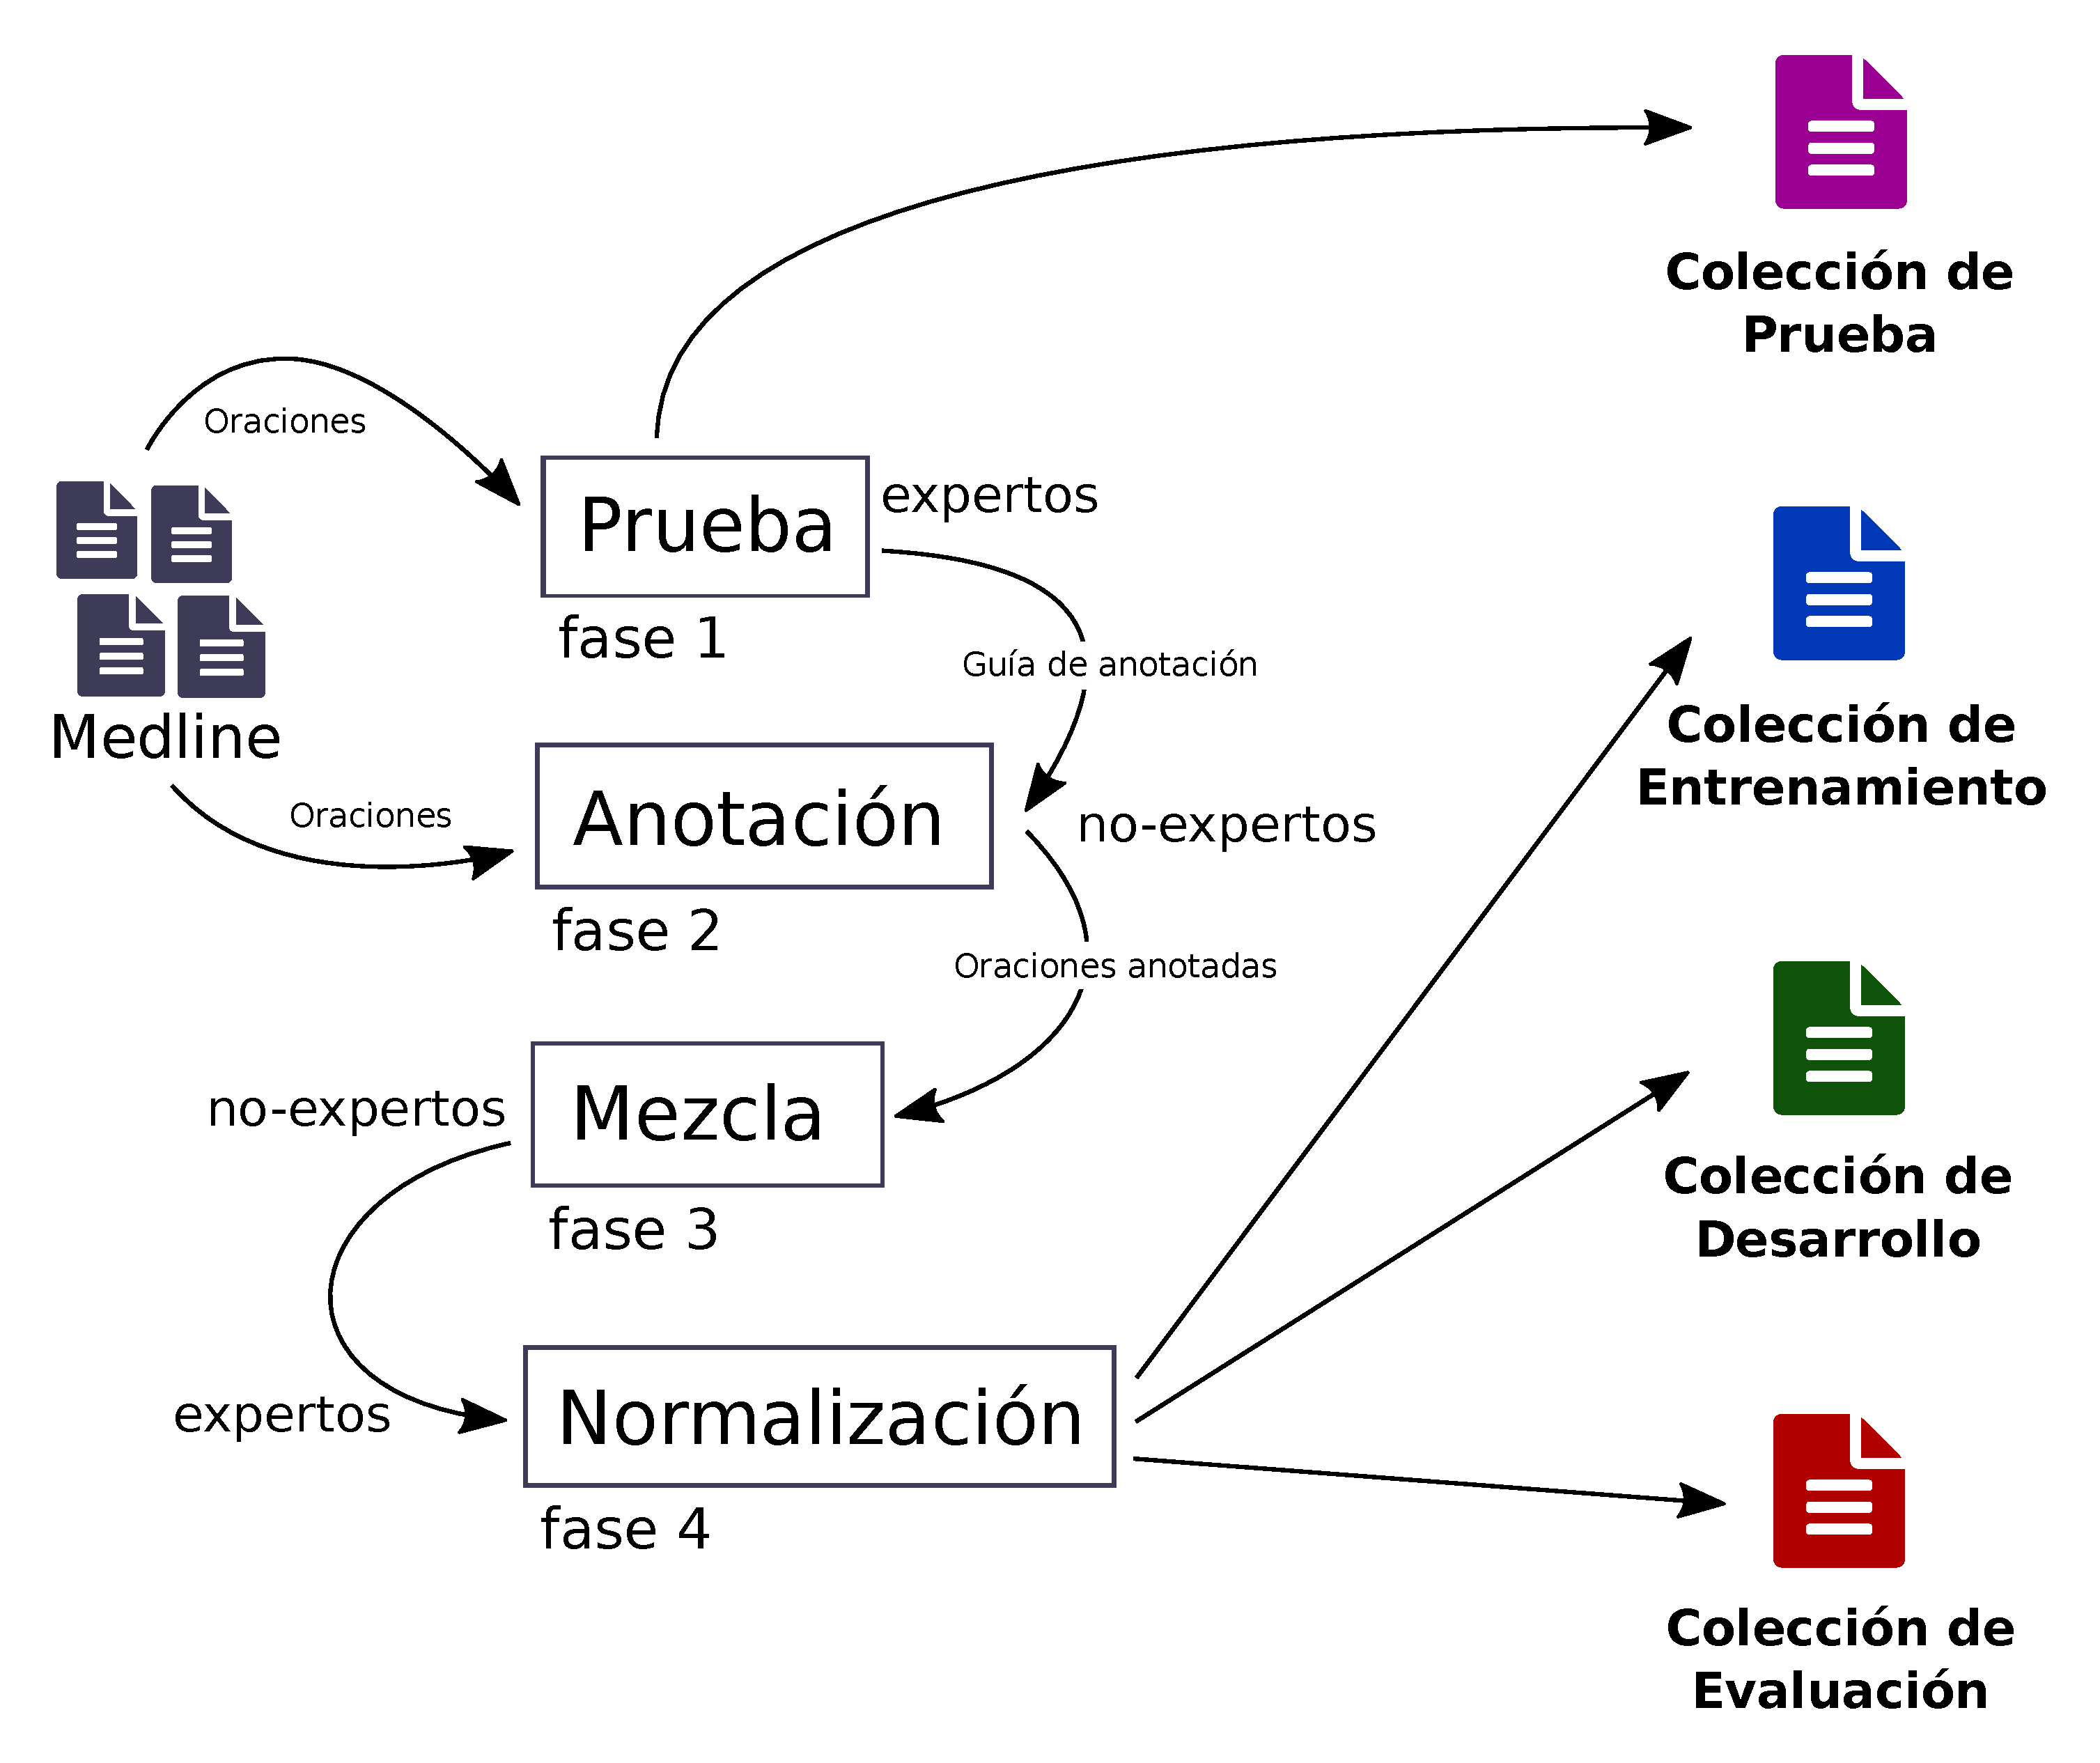
\includegraphics[width=0.9\textwidth]{Images/Chapters/AnnotationProcess.pdf}
    \caption{Esquema general del proceso de anotación.}
    \label{fig:annotation-process}
\end{figure}

La Figura~\ref{fig:annotation-process} describe el proceso de anotación seguido en todos los corpus desarrollados en esta investigación, consistente en 4 etapas fundamentales. En primer lugar un conjunto reducido de anotadores expertos
construye una colección de prueba con un número pequeño de oraciones~(p.e., 50 oraciones), escogidas específicamente
para cubrir la mayor cantidad posible de patrones de anotación. Con esta colección se construye una guía de anotación que se distribuye entre un conjunto de anotadores no-expertos para su entrenamiento y evaluación. Los anotadores no-expertos realizan la anotación manual del resto del corpus, de forma que cada oración es anotada por exactamente dos personas diferentes sin interacción entre sí.
Luego se realiza un proceso de mezcla para escoger entre las 2 versiones anotadas de cada oración.
Para cada oración anotada, esta mezcla la realiza respectivamente uno de los anotadores no-expertos que no haya participado en la primera fase en dicha oración. De esta forma cada oración ha sido evaluada hasta este paso por 3 personas diferentes.
Finalmente, los anotadores expertos revisan en conjunto todas las oraciones anotadas y proponen modificaciones menores que deben ser aprobadas por unanimidad.

\todo{Poner citas a Zenodo de los corpus}
Siguiendo este proceso de anotación y el esquema definido en la Sección~\ref{results:schema}, se han construido 3 corpus de tamaño similar, utilizados respectivamente como escenarios de evaluación en las ediciones 2018, 2019 y 2020 del \textit{eHealth-KD Challenge}.
Aunque la composición exacta del comité de anotadores no-expertos ha variado en cada uno de los corpus, el conjunto de anotadores expertos se ha mantenido constante, y la mayoría de los anotadores no-expertos han participado en más de uno de los corpus.
En las tres ediciones el grueso de las oraciones se han obtenido de la base de datos \textit{Medline Plus}\footnote{\url{https://medlineplus.gov/xml.html}} que contiene artículos en idioma español (además de inglés) en el dominio de la salud. En la edición 2020 se adicionó como fuente de información un conjunto de $200$ artículos seleccionados aleatoriamente de \textit{Wikinews} para estimular el desarrollo de sistemas de aprendizaje multi-dominio y evaluar cuán generalizable es el esquema de anotación.
Todas las oraciones anotadas son en idioma español.

La Tabla~\ref{tab:corpus} resume las estadísticas fundamentales de los tres corpus anotados, denominados
respectivamente \textit{eHealth-KD} 2018, 2019 y 2020.
El corpus de la edición 2018~(ver Capítulo~\ref{Chap:CorpusV1}) fue anotado con una versión simplifica del esquema de anotación, dado que aún no se había formalizado completamente. Por este motivo solamente se anotaron acciones, conceptos, y 4 relaciones semánticas. En total se anotaron $1,173$ oraciones que agrupan $13,113$ elementos semánticos.
En la edición 2019~(ver Capítulo~\ref{Chap:CorpusV2}) se introdujeron todos los elementos semánticos del esquema de anotación y se anotaron $1,045$ oraciones nuevas con un total de $13,246$ elementos.
Para la edición 2020 se reutilizaron $1,000$ oraciones de la edición anterior, y se adicionaron $500$ oraciones nuevas siguiendo el mismo esquema de anotación, $300$ de dominio médico y $200$ de artículos periodísticos.
En total se han anotado $2,718$ oraciones en idioma español con $34,897$ elementos semánticos que capturan múltiples patrones lingüísticos en documentos del dominio médico y periodístico.

\begin{table}[tpb]
    \centering
    \resizebox{!}{0.425\textheight}{
    \begin{tabular}{lrrrr}
    \toprule
         & \multicolumn{3}{c}{\textbf{Corpus eHealth-KD}} \\
         & \textbf{2018} & \textbf{2019} & \textbf{2020} & \textbf{Total} \\
    \midrule
        \textit{Oraciones}          &        1,173      & 1,045  & ${}^*$1,500  & 2,718  \\
        \,\,\,Prueba                &           29      &  45    & 0            & 74     \\
        \,\,\,Entrenamiento         &          559      & 600    & ${}^*$800    & 1,159  \\
        \,\,\,Desarrollo            &          285      & 100    & ${}^*$200    & 385    \\
        \,\,\,Evaluación            &          300      & 300    & 500          & 1,100  \\
    \midrule
        \textit{Anotaciones}        &        13,113     & 13,246 & 8,538        & 34,897 \\
    \midrule
        \textit{Entidades}          &        7,188      & 6,612 &  4,237        & 18,037 \\
          \texttt{ Concept}         &        5,366      & 4,092 &  2,803        & 12,261 \\
          \texttt{ Action}          &        1,822      & 1,742 &  944          & 4,508  \\
          \texttt{ Predicate}       &           -       & 563   &  420          & 983    \\
          \texttt{ Reference}       &            -      & 215   &  70           & 285    \\
    \midrule
        \textit{Relaciones}         &       5,925       & 6,049 &  4,037        & 16,011 \\
          \texttt{ target}          &       2,120       & 1,729 &  855          & 4,704  \\
          \texttt{ subject}         &       1,466       & 894   &  706          & 3,066  \\
          \texttt{ is-a}            &       1,057       & 566   &  383          & 2,006  \\
          \texttt{ part-of}         &       393         & 94    &  57           & 544    \\
          \texttt{ has-property}    &       836         & 159   &  111          & 1,006  \\
          \texttt{ same-as}         &        53         & 124   &  85           & 262    \\
          \texttt{ in-context}      &         -         & 677   &  584          & 1,261  \\
          \texttt{ in-place}        &         -         & 400   &  351          & 751    \\
          \texttt{ in-time}         &         -         & 165   &  215          & 380    \\
          \texttt{ domain}          &         -         & 364   &  285          & 649    \\
          \texttt{ argument}        &         -         & 343   &  233          & 576    \\
          \texttt{ causes}          &         -         & 367   &  131          & 498    \\
          \texttt{ entails}         &         -         & 167   &  41           & 208    \\
    \midrule
        \textit{Attributos}         &         -         & 585   & 264           & 849    \\
          \texttt{ diminished}      &         -         &  18   & 11            & 29     \\
          \texttt{ emphasized}      &         -         & 124   & 80            & 204    \\
          \texttt{ negated}         &         -         & 164   & 72            & 236    \\
          \texttt{ uncertain}       &         -         & 279   & 101           & 380    \\
    \bottomrule
    \end{tabular}}
    \caption[Estadísticas del corpus \textit{eHealth-KD}.]{Estadísticas de las 3 ediciones del corpus \textit{eHealth-KD}. Los números anotados con ${}^*$ en 2020 indican que se han reutilizado $1000$ oraciones de la edición 2019. En este caso solo se contabilizan las anotaciones correspondientes a las $500$ oraciones nuevas.}
    \label{tab:corpus}
\end{table}

\section{Definición de Tareas}\label{results:tasks}

Los recursos lingüísticos presentados en la Sección~\ref{results:corpus} son necesarios para entrenar sistemas computacionales que sean capaces de extraer automáticamente contenido semántico de lenguaje natural. Para avanzar en esta tarea es conveniente diseñar un entorno de evaluación que permita comparar de forma objetiva los enfoques posibles. Para evaluar mejor las fortalezas y debilidades de los diferentes enfoques, la tarea de anotación automática se divide en dos subtareas:

\begin{description}
    \item[Subtarea A: Reconocimiento de Entidades.]
    El propósito de esta subtarea es identificar todas las entidades mencionadas en una oración y sus clases correspondientes.~(i.e., \texttt{Concept}, \texttt{Action}, \texttt{Predicate} y \texttt{Reference}.

    \item[Subtarea B: Extracción de relaciones.]
    El propósito de esta subtarea es detectar todas las relaciones semánticas entre cada par de entidades ya etiquetadas en cada oración.
\end{description}

Como criterio de evaluación de ambas subtareas se propone una versión extendida de la métrica $F_1$ modificada para tratar coincidencias parciales. La métrica $F_1$ depende de las anotaciones correctas, incorrectas, parciales, faltantes y espurias en todo el conjunto de evaluación. Dependiendo de la(s) subtarea(s) bajo evaluación, definimos los siguientes tipos de resultados:

\begin{description}
\item[Subtarea A - Correctos $C_A$:] cuando una anotación coincide exactamente con la anotación correcta correspondiente.
\item[Subtarea A - Incorrectos $I_A$:] cuando una anotación coincide con una anotación correcta con respecto al espacio de texto pero define una etiqueta de entidad diferente.
\item[Subtarea A - Parciales $P_A$:] cuando un fragmento de texto tiene una intersección no vacía pero inexacta con una anotación correcta, como el caso de ``\textit{vías respiratorias}'' y ``\textit{vías}'' en la Figura~\ref{fig:example}, oración 2.
Las frases parciales solo se comparan con una frase correcta~(es decir, la primera frase parcialmente coincidente desde el principio de la oración) para evitar que algunos fragmentos de texto grandes que cubren la mayor parte del documento obtengan una puntuación muy alta.
\item [Subtarea A - Faltantes $M_A$:] cuando no se produce una anotación que aparece en la colección de anotaciones correctas.
\item [Subtarea A - Espurios $S_A$:] cuando se produce una anotación que no aparece en la colección de anotaciones correctas.
\end{description}

\begin{description}
\item[Subtarea B - Correctos $C_B$:] cuando existe una relación entre dos entidades en la colección de anotaciones correctas.
\item[Subtarea B - Faltantes $M_B$:] cuando no se produce una relación en la colección de anotaciones correctas.
\item[Subtarea B - Espurios $S_B$:] cuando se produce una relación pero no aparece en la colección de anotaciones correctas.
\end{description}

Se define $Precision$, $Recall$, y $F_1$ de la manera usual, teniendo en cuenta que para cada escenario de evaluación solo se consideran los términos relacionados con la(s) subtarea(s) bajo evaluación.

\begin{eqnarray}
Precision & = & \frac{C_A + C_B + \frac{1}{2} P_A}{C_A + I_A + C_B + P_A + S_A + S_B} \\
Recall    & = & \frac{C_A + C_B + \frac{1}{2} P_A}{C_A + I_A + C_B + P_A + M_A + M_B} \\
F_1       & = & 2 \cdot \frac{Precision \cdot Recall}{Precision + Recall} \label{eqn:f1}
\end{eqnarray}{}

Finalmente, se propone $F_1$ como se define en la Ecuación~\ref{eqn:f1} como la métrica oficial para comparar diferentes enfoques. En cada versión del corpus \textit{eHealth-KD} se define un subconjunto diferente de oraciones para evaluar cada subtarea de forma independiente o ambas tareas de manera simultánea.

\section{Infraestructura de Aprendizaje y Evaluación}\label{results:infrastructure}

Para apoyar a los investigadores en el desarrollo de tecnologías de descubrimiento de conocimiento, se proporciona un conjunto de herramientas e infraestructura que permiten un proceso de experimentación más rápido y objetivo.
Estos recursos están disponibles gratuitamente para la comunidad científica en una colección de repositorios de Github\footnote{\url{https://ehealthkd.github.io}}.\todo{Mover a Github}
El conjunto de recursos desarrollado consiste en los siguientes elementos:

\begin{itemize}
\item Archivos de texto plano y anotaciones en formato BRAT Standoff~\cite{brat} para el corpus \textit{eHealth-KD}, dividido en colecciones de entrenamiento, desarrollo y evaluación.
\item Archivos de configuración necesarios para desplegar un servidor BRAT con el objetivo de analizar y ampliar el corpus \textit{eHealth-KD}, o para crear otros recursos lingüísticos basados en el esquema de anotación descrito en la Sección~\ref{results:schema}.
\item Herramientas en el lenguaje de programación Python para cargar y manipular las anotaciones de BRAT Standoff así como para producir resultados formateados correctamente.
\item Herramientas para configurar y ejecutar algoritmos de evaluación para la tarea definida en la Sección~\ref{results:tasks}, incluidas las subtareas, y calcular las métricas de evaluación oficiales.
\item Un conjunto de implementaciones de algoritmos de aprendizaje básicos con diferentes grados de complejidad, incluida una estrategia aleatoria y varios enfoques clásicos.
\end{itemize}

Usando las herramientas antes mencionadas, los investigadores pueden desarrollar rápidamente nuevos enfoques extendiendo las implementaciones \textit{baseline} o desarrollando una solución desde cero, sin tener que lidiar con la configuración del entorno o la implementación de las métricas de evaluación.
Además de poder evaluar sus soluciones personalmente, los investigadores también pueden subir
sus soluciones a un entorno de evaluación en la nube y obtener automáticamente las métricas relevantes
así como comparar sus resultados con soluciones ya publicadas.
Se mantiene una tabla de clasificación oficial que sirve como un estado del arte actualizado en todas las subtareas.
Esta información contiene no solo los resultados numéricos, sino también información estructurada sobre los enfoques utilizados y enlaces a las publicaciones relevantes\footnote{\url{https://ehealthkd.github.io/results}}.

\section{Evaluación de Sistemas}\label{results:challenge}

Las tres versiones del corpus \textit{eHealth-KD} presentadas en la Sección~\ref{results:corpus} han sido utilizadas en la evaluación de sistemas de extracción de conocimiento diseñados por diversos equipos de investigadores en el marco del evento \textit{eHealth Knowledge Discovery}, organizado en los años 2018, 2019 y 2020. En la Tabla~\ref{tab:results-challenge} se resumen los resultados más importantes de las 3 ediciones de este evento. Se reportan el número de participantes (equipos de investigadores), los mejores resultados alcanzados tanto en el proceso completo de extracción como en cada una de las subtareas definidas en la Sección~\ref{results:tasks}~(en términos de la métrica $F_1$), así como un resumen de las técnicas más utilizadas.

\begin{table}[htb]\centering
    \begin{tabular}{lrrr}
        \toprule
        	                             &\bf 2018	&\bf 2019	&\bf 2020	\\
        \midrule
            Equipos Registrados          &	31  	&	30	    &	26  	\\
            Equipos Participantes        &	6	    &	10	    &	8	    \\
        \midrule
            Resultados generales         &	0.744	&	0.639	&	0.660	\\
            Subtarea A (entidades)       &	0.872	&	0.820   &	0.825	\\
            Subtarea B (relaciones)      &	0.448	&	0.626	&	0.633	\\
        \midrule
            \textbf{Técnicas}            &	    	&	    	&		    \\
            PLN clásico                  &	5	    &	7   	&	0	    \\
            Reglas	                     &	2	    &	2   	&	3	    \\
            \textit{Embeddings}          &	2	    &	7   	&	8   	\\
            Redes neuronales         	 &	3   	&	10  	&	7   	\\
            \textit{Transformers}        &	0   	&	1   	&	5   	\\
            Conocimiento externo    	 &	2   	&	1   	&	3   	\\
            Solución \textit{end-to-end} &	0   	&	1   	&	2   	\\
        \bottomrule
    \end{tabular}
    \caption[Resultados del \textit{eHealth Knowledge Discovery}]{Resumen de los resultados de las tres ediciones del \textit{eHealth Knowledge Discovery} y las técnicas más comúnmente aplicadas en cada edición.\label{tab:results-challenge}
}\end{table}

Con respecto a los resultados obtenidos en la solución de las tareas, es necesario reconocer que la complejidad de la edición 2018 es significativamente menor debido a que existe un menor número de tipos de entidades y relaciones. Por este motivo los resultados no son directamente comparables con los de las ediciones 2019 y 2020. Aún así, una posible conclusión de estos resultados es que la detección de entidades está de manera general resuelta mientras que la extracción de relaciones consiste en el mayor reto.

Analizando las técnicas más utilizadas por los sistemas presentados en cada edición, se puede notar una tendencia hacia los sistemas \textit{end-to-end} basados en arquitecturas de redes neuronales, o sea, sistemas que resuelven ambas tareas como parte de una misma arquitectura en vez de como pasos separados.
De manera general las redes neuronales, y en particular los \textit{embeddings}~(e.g., word2vec, glove) y las arquitecturas \textit{transformer}~(e.g., BERT, GPT), han reemplazado a las técnicas clásicas de procesamiento de lenguaje natural. Sin embargo, aún es necesario el uso de ciertas reglas específicas del dominio, por ejemplo, para resolver el problema de las entidades superpuestas. Por otro lado, los enfoques que aprovechan conocimiento externo, aunque no son mayoría siguen teniendo importancia, fundamentalmente en la forma de \textit{embeddings} de dominio específico.

\section{Anotación Asistida}\label{results:assisted-ann}

El proceso de anotación, mezcla y normalización que se ha llevado a cabo durante el transcurso de esta investigación ha permitido reconocer la importancia de esta fase como parte del desarrollo de sistemas de aprendizaje automático y descubrimiento de conocimiento.
La construcción de recursos lingüísticos anotados por expertos es fundamental para entrenar este tipo de sistemas, y consiste en una de las tareas más costosas en términos de esfuerzo humano.
Además, si no se cuenta con una planificación ideal, es probable que los recursos creados sean menos efectivos. Por ejemplo, pueden contener oraciones repetidas o semánticamente similares, conjuntos desbalanceados de etiquetas, y contradicciones internas.
Una forma de aliviar estos problemas y acelerar el proceso de anotación es introducir un mecanismo de aprendizaje automático dentro del propio ciclo de anotación, mezcla y normalización, que ayude a seleccionar los mejores ejemplos a anotar y garantice que no existe redundancia innecesaria en el corpus.

Como parte de esta investigación se propone una estrategia de aprendizaje activo diseñada para un corpus arbitrario de oraciones en lenguaje natural, cada una de las cuales debe ser anotada por un experto humano a nivel semántico, tal y como ocurre con el esquema de anotación propuesto en la Sección~\ref{results:schema}.
Con el objetivo de diseñar una propuesta generalizable, se considera un conjunto arbitrario $\mathcal{E}$ de etiquetas de entidades, cada una de las cuales puede abarcar uno o más tokens, continuos o discontinuos,
y un conjunto predefinido $\mathcal{R}$ de tipos de relaciones binarias entre entidades.
Este modelo de anotación abstracto puede representar una amplia gama de tareas diferentes, incluyendo el corpus \textit{eHealth-KD} en el cuál se inspira, pero abarcando además desde la extracción de relaciones de  dominio específico (por ejemplo, interacción gen-proteína) hasta la representación semántica de propósito general (por ejemplo, análisis de AMR).
Esta estrategia se describe en detalle en el Capítulo~\ref{Chap:Annotation}.

\begin{figure}[htb]
    \centering
    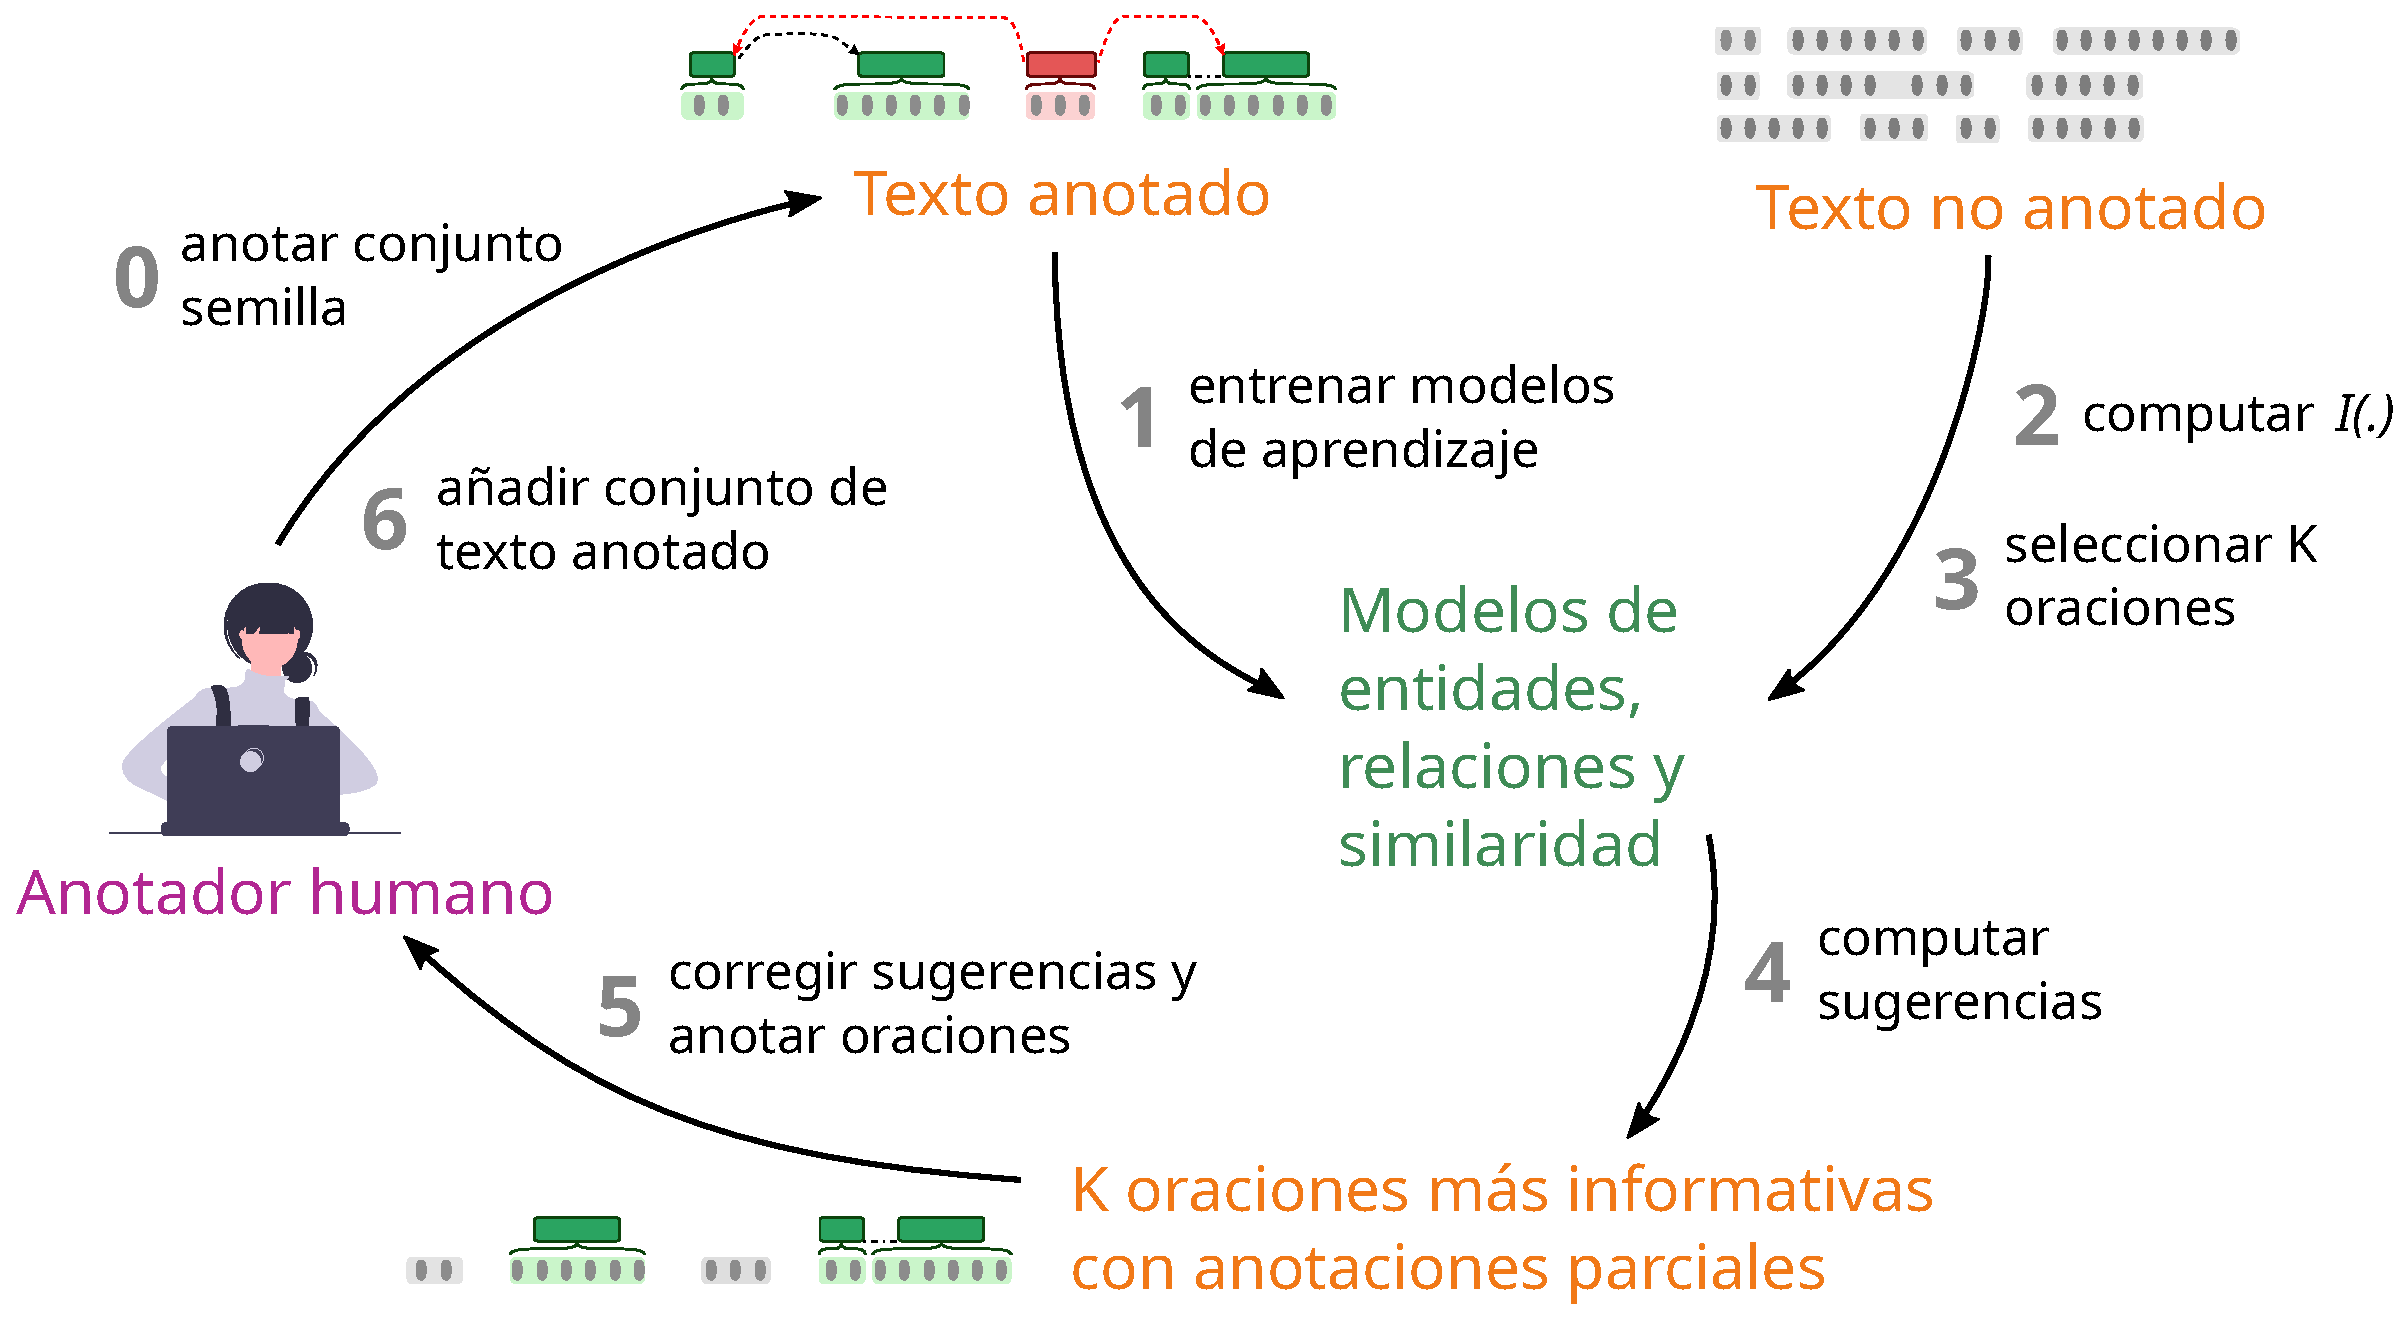
\includegraphics[width=\textwidth]{Images/Chapters/SchemaAssistedAnnotation.pdf}
    \caption[Estrategia de aprendizaje activo.]{Ilustración de alto nivel de la estrategia de aprendizaje activo presentada en esta investigación para la anotación asistida del corpus ehealth-KD.}
    \label{fig:model}
\end{figure}

\newcommand{\Labeled}{\mathbf{L}}
\newcommand{\Unlabeled}{\mathbf{U}}
\newcommand{\infr}[1]{I(#1)}
\newcommand{\infrc}{\infr{\cdot}}
\newcommand{\unc}[1]{H(#1)}
\newcommand{\uncc}{\unc{\cdot}}
\newcommand{\id}[1]{ID(#1)}
\newcommand{\uncm}[1]{\hat{H}(#1)}
\newcommand{\unccm}{\uncm{\cdot}}

La estrategia de aprendizaje activo propuesta en esta investigación funciona de forma iterativa en lotes de $K$ oraciones~(por ejemplo, $K=10$).
En cada iteración, existe un conjunto etiquetado $\Labeled$ con $|\Labeled|=n \times K$ oraciones anotadas manualmente por un anotador humano, y un conjunto mayor  $\Unlabeled$ de oraciones no etiquetadas.
Inicialmente, el anotador humano selecciona $K$ oraciones representativas y realiza una anotación manual completa~(paso 0).
Posteriormente, dos modelos de aprendizaje automático se entrenan iterativamente en las oraciones etiquetadas manualmente~(paso 1) y una métrica de \textit{informatividad}, $\infr{s}$, se calcula para cada oración $s \in \Unlabeled$~(paso 2).
Las mejores oraciones $K$ en términos de $\infrc$ se seleccionan~(paso 3) y el modelo produce una predicción de entidades y relaciones para cada una~(paso 4).
Cada predicción tiene una métrica de \textit{incertidumbre} asociada, $\uncc$, estimada por los modelos.
En función de esta incertidumbre y umbrales predefinidos $u_e$ y $u_r$ para entidades y relaciones respectivamente, todas las entidades $e_i$ (relaciones $r_j$) con una incertidumbre estimada $\unc{e_i}>u_e$ ($\unc{r_j}>u_r$) se descartan.
Finalmente, las oraciones seleccionadas y parcialmente anotadas se presentan al anotador humano, quien debe corregir las anotaciones incorrectas y agregar las anotaciones faltantes~(paso 5).
Las oraciones corregidas se incorporan al grupo etiquetado para la siguiente iteración~(paso 6).

Para estimar la informatividad $\infr{s_i}$ de cada oración $s_i \in \Unlabeled$, se define una métrica basada en el modelo de \textit{uncertainty sampling}~\cite{settles2008analysis}.
Dado un conjunto de $n$ anotaciones de entidades $E_i \subseteq \mathcal{E}^n = \{ e^i_1, \ldots, e^i_n \}$ y $m$ anotaciones de relaciones $R_i \subseteq \mathcal{R}^m = \{ r^i_1, \ldots, r^i_m \}$ producidas para una oración $s_i$, se define la incertidumbre de cada entidad $e^i_k$ (o relación $r^i_k$) como la entropía de la distribución de probabilidades de cada una de las posibles etiquetas para dicha entidad o relación. Formalmente:

\small
$$
\unc{e^i_k} = -\sum_{l_j \in \mathcal{E}} P(e^i_k=l_j | s_i;\theta) \log_2 P(e^i_k=l_j | s_i;\theta)
$$
$$
\unc{r^i_k} = -\sum_{l_j \in \mathcal{R}} P(r^i_k=l_j | s_i;\theta) \log_2 P(r^i_k=l_j | s_i;\theta)
$$
\normalsize

\noindent
Donde $\theta$ representa los parámetros del modelo de aprendizaje que se utiliza para estimar estas probabilidades.

De la misma forma se puede definir la incertidumbre media asociada a las entidades y relaciones producidas, respectivamente:

\small
$$
\uncm{E_i} = \frac{1}{n} \sum_{e^i_k \in E_i} \unc{e^i_k} \,\,\,\,\,\,\,\, \uncm{R_i} = \frac{1}{m} \sum_{r^i_k \in R_i} \unc{r^i_k}
$$
\normalsize

Además, se define una métrica de densidad de información $\id{s_i}$ para estimar cuán representativa es cada oración $s_i$
con respecto al conjunto de oraciones anotadas. De forma similar a~\citet{settles2008analysis},
$\id{s_i}$ se define como la similaridad promedio de la oración $s_i$ a un conjunto $K$ de oraciones anotadas:

\small
$$
\id{s_i} = \frac{1}{K} \sum_{s_j \in \Labeled_i^*} sim(s_i, s_j)
$$
\normalsize

\noindent Donde $\Labeled_i^*$ es el subconjunto de las $K$ oraciones anotadas que maximizan la similaridad con respecto a $s_i$. Cualquier métrica de similaridad podría ser utilizada, pero en esta investigación se propone usar \textit{embeddings} de \textit{Doc2Vec}~\cite{doc2vectgensim}
pre-entrenados en el conjunto $\Unlabeled$ de oraciones no anotadas.

Finalmente, la \textit{informatividad} total de una oración no anotada $s_i$ se estima a partir de la incertidumbre de cada componente (entidad o relación) ponderados por la densidad de información de la oración:

\small
$$
\infr{s_i} = \left[ \uncm{E_i} + \uncm{R_i} \right] \times \id{s_i}^{\beta}
$$
\normalsize

Para evaluar la efectividad de este enfoque se simula el proceso de anotación asistida en el corpus \textit{eHealth-KD} 2019, comparando las estrategias de aprendizaje activo con la anotación en el orden original sin sugerencias~(como modelo de base).
Como el proceso de anotar un corpus es costoso, la simulación se basa en las anotaciones correctas de la colección de entrenamiento.
La mejora se puede estimar comparando cuántas oraciones necesitan anotaciones para alcanzar un rendimiento específico de los algoritmos de aprendizaje automático~(medido en términos de $F_1$ en la colección de pruebas).

Para ilustrar el grado de reducción de tiempo alcanzado, la Figura~\ref{fig:graph2} muestra el número mínimo de oraciones que deben anotarse para alcanzar diferentes puntajes relativos de $F_1$.
Por ejemplo, después de anotar las primeras $400$ oraciones, es posible lograr un $95\%$ del resultado final de $F_1$ cuando se utiliza todo el corpus.
Sin embargo, para alcanzar la puntuación objetivo, las primeras $880$ oraciones de las $1000$ totales deben anotarse si el corpus se anota en el orden original~(seguido por el modelo de base).
Por el contrario, la estrategia de aprendizaje activo solo requiere anotar entre $530$ y $580$ oraciones para alcanzar el mismo valor de $F_1$, ahorrando así entre $35\%$ y $40\% $ del tiempo de anotación humano.

\begin{figure}[tb]
    \centering
    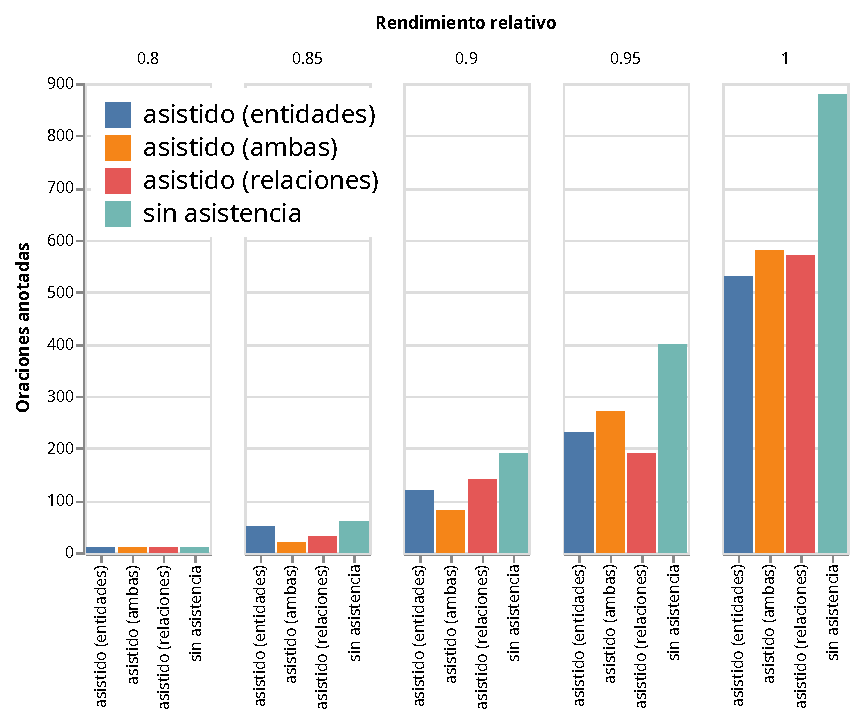
\includegraphics[width=0.8\columnwidth]{Images/Chapters/CostReductionAssistedAnnotation.pdf}
    \caption[Evaluación de la estrategia de aprendizaje activo]{Número mínimo de oraciones necesarias para alcanzar un rendimiento específico en relación con la métrica $F_1$ con cada estrategia de aprendizaje activa para la sugerencia de oraciones.}
    \label{fig:graph2}
\end{figure}

Otro análisis interesante es estimar hasta qué punto las anotaciones sugeridas reducen aún más el tiempo total de anotación.
Un anotador humano que use esta herramienta deberá aceptar algunas de las anotaciones sugeridas, corregir las incorrectas y anotar las faltantes.
Cada una de estas acciones tiene un costo diferente.
Para cuantificar la mejora en el tiempo general que producen las sugerencias, se asigna un costo relativo~(en términos de unidades de tiempo abstractas) a cada uno de los siguientes tipos de anotaciones:

\begin{description}
    \item [Faltantes:] 1 unidad de tiempo.
    \item [Espurias:] 2 unidades de tiempo.
    \item [Correctas:] 0.25 unidades de tiempo.
    \item [Parciales:] 0.5 unidades de tiempo.
\end{description}

Esta estructura de costos asume que el problema de corregir anotaciones incorrectas es más complejo que simplemente producir las anotaciones correctas, al tiempo que reconoce que incluso estar de acuerdo con las anotaciones correctas tiene un costo.
Para que una estrategia de aprendizaje activo sea útil, debe proporcionar suficientes anotaciones correctas para superar el costo de corregir las anotaciones incorrectas; por lo tanto, debe priorizar la precisión sobre el recobrado.
Una simulación de este proceso para diferentes valores de los umbrales de incertidumbre arroja que, en el caso óptimo, se reduce a un $76\%$ el costo de arreglar una oración parcialmente anotada con respecto a la anotación manual.

Se puede estimar una reducción general en el tiempo de anotación para esta simulación experimental combinando las mejoras proporcionadas por las sugerencias de anotación y el orden de las oraciones.
Asumiendo que ambos efectos son independientes, el mejor de los casos para este corpus sugiere lo siguiente.
Usando el enfoque de aprendizaje activo, un anotador humano habría necesitado anotar solo $530$ oraciones de $ 1000$, cada una de ellas con un costo de tiempo estimado de $76\%$ en comparación con la anotación completa.
Esto da como resultado una reducción general de hasta $60\%$ del tiempo de anotación total, produciendo un corpus más pequeño en el que los modelos de aprendizaje automático aún pueden ser entrenados, ofreciendo el mismo rendimiento que los modelos entrenados en el corpus original.

\section{Discusión}
\label{chap2:discussion}

Esta sección presenta una discusión general de las principales contribuciones de esta investigación, las lecciones aprendidas y las limitaciones de las soluciones actuales propuestas para la tarea \textit{eHealth Knowledge Discovery}. También se destacan ideas interesantes para la investigación futura, basadas en los conocimientos obtenidos al analizar los enfoques más prometedores.

\subsection{Contribuciones}

Se han desarrollado diferentes representaciones semánticas para capturar el conocimiento expresado en lenguaje natural~(p.e., AMR, FrameNet y PropBank).
El principal inconveniente de estas representaciones es su complejidad, ya que a menudo dependen de lexicones que definen los roles semánticos específicos para cada palabra.
Por lo tanto, desarrollar sistemas de inteligencia artificial para el descubrimiento del conocimiento con este nivel de detalle es aún un problema no resuelto.
El uso de representaciones semánticas más simples, que no se basen en roles o relaciones específicas, puede simplificar el desarrollo de técnicas basadas en el aprendizaje automático.

Esta investigación propone una línea de desarrollo en esta dirección, donde el descubrimiento de conocimiento con un alto nivel de abstracción pueda ser refinado posteriormente para tareas de dominio específico.
El propósito no es reemplazar las representaciones semánticas detalladas, como AMR o FrameNet, sino proporcionar una representación más general que se pueda usar como un paso inicial en diferentes tareas de descubrimiento de conocimiento.
Este tipo de representación semántica puede simplificar tareas posteriores como el aprendizaje de ontologías, de la misma manera que el etiquetado POS-tag de propósito general a menudo se realiza antes de tareas de PLN más complejas.
Basado en las experiencias obtenidas durante el proceso de anotación, mezcla y normalización, se ha diseñado un mecanismo para la anotación semi-automática.
En los experimentos realizados se pudo comprobar cómo utilizando modelos de aprendizaje relativamente sencillos se puede acelerar considerable el proceso de anotación.

Los recursos, herramientas e infraestructura desarrollados en esta investigación tienen como objetivo proporcionar una base para que la comunidad científica construya técnicas de descubrimiento de conocimiento de propósito general.
Progresar en esta dirección depende no solo de los avances teóricos, como mejores arquitecturas de aprendizaje profundo o técnicas de procesamiento del lenguaje natural, sino también de la disponibilidad de recursos que permitan una experimentación eficiente.
En este sentido, esta propuesta introduce una nueva tarea de descubrimiento de conocimiento así como métricas de evaluación formalmente definidas y un conjunto de evaluación práctico donde los investigadores pueden desarrollar rápidamente nuevas técnicas y obtener retroalimentación inmediata.
También es un paso en la dirección de alentar la investigación de descubrimiento de conocimiento en idiomas menos utilizados, como el español, y en dominios socialmente importantes como la salud, así como evaluar las capacidades de generalización de los sistemas existentes a múltiples dominios.

\subsection{Desafíos actuales y futuros}

Los resultados de las tres ediciones del evento \textit{eHealth-KD} permiten analizar sobre la complejidad de los diversos pasos involucrados en el diseño de sistemas de descubrimiento automático de conocimiento para esta tarea.
La mayoría de los sistemas modelaron la tarea como una secuencia en la que se reconocen primero las entidades y luego se extraen las relaciones. La subtarea A se modela comúnmente como un problema de etiquetado de secuencia y se resuelve mediante técnicas estándar, por ejemplo, redes Bi-LSTM y CRF. La subtarea B se modela comúnmente como un problema de clasificación estándar, donde la entrada consiste en una representación del un par de conceptos, utilizando \textit{embeddings} contextuales y otras características sintácticas.
Sin embargo, algunos de los sistemas de mejor desempeño en las últimas ediciones del \textit{eHealth Knowledge Discovery} consisten en enfoques \textit{end-to-end} que predicen las entidades y relaciones simultáneamente.
Además de diferencias marginales en las arquitecturas y las metodologías de entrenamiento, argumentamos que la fortaleza de estos sistemas surge del efecto de regularización del aprendizaje de una representación unificada para ambas subtareas, en lugar de diferentes representaciones, lo que permite obtener más información de la misma cantidad de datos de entrenamiento.

En base a estas observaciones, estimamos que los enfoques más efectivos para este problema deberían considerar las siguientes estrategias:
resolver ambos problemas simultáneamente en lugar de secuencialmente; usando \textit{embeddings} pre-entrenados de propósito general o contextuales en lugar de \textit{embeddings} personalizados; aplicar técnicas de ampliación del conjunto de datos para incrementar la cobertura estadística; y, diseñar reglas específicas para lidiar con la superposición y la discontinuidad de entidades.

En comparación con el nivel de experticia humano, la subtarea B parece ser considerablemente más difícil para los sistemas de aprendizaje automático que para los humanos. En experimentos reportados en el Capítulo~\ref{Chap:CorpusV2}, un anotador experto supera al sistema con el mejor rendimiento en un total de $8.8$\% en la tarea completa, pero solo en un $4.1$\% en la subtarea A, en comparación con un $10.9$\% en la subtarea B. Intuitivamente, la subtarea B debería ser más difícil, ya que el número de etiquetas para predecir es mayor que en la subtarea A. Sin embargo, esto no explica la diferencia en el rendimiento entre humanos
y sistemas de aprendizaje automático. En promedio, los sistemas que intentan resolver la subtarea B obtienen un valor $F_1$ a menudo significativamente menor en la subtarea B en comparación con la tarea completa, mientras que el anotador experto es ligeramente mejor en la subtarea B. Esto indica que los humanos pueden obtener conocimiento adicional al ver las anotaciones correctas para la subtarea A que los sistemas de aprendizaje automático no reconocen.
Sin embargo, el hecho de que la subtarea B sea significativamente más difícil para los humanos que la subtarea A es una indicación del alto grado de análisis cualitativo involucrado en este problema. Como tal, hay un umbral por encima del cual incluso los expertos humanos no estarán completamente de acuerdo, dada la naturaleza inherentemente subjetiva de la comprensión del lenguaje natural.

La aparición de las arquitecturas \textit{Transformer} y su éxito reciente en varias tareas de PLN~\cite{bert} abre las puertas a mejorar potencialmente los resultados actuales con poco esfuerzo adicional. La primera edición del evento~(en 2018) consistió principalmente en sistemas híbridos, usando una combinación de técnicas de PLN basadas en reglas y conocimiento externo con aprendizaje automático. Sin embargo, la edición de 2019 no incluyó casi ningún enfoque basado en reglas, en favor de arquitecturas de aprendizaje profundo más complejas, y en la edición del 2020 se destacó el uso de \textit{Transformers} combinados con diseños de arquitecturas específicas para cada subtarea.

Sin embargo, se aprecia que todavía hay un gran margen de mejora a través de enfoques que consideren la información global de la oración completa en lugar de simplificar el problema como un conjunto de subtareas de clasificación independientes. Desde una perspectiva humana, la anotación de una oración es un proceso global, en el que la decisión de considerar una palabra específica como \texttt{Action} o \texttt{Predicate} hace que un anotador reconsidere la oración completa y potencialmente cambie otras anotaciones. La incorporación de este tipo de conciencia global en un sistema requiere más que \textit{embeddings} contextuales o incluso modelos de lenguaje a nivel de oración. El sistema debe poder evaluar una oración anotada de manera incompleta y potencialmente deshacer o corregir etiquetas anteriores a medida que avanza, hasta que se alcance un criterio de convergencia adecuado. Este tipo de comportamiento requiere un marco más expresivo que el que ofrecen las arquitecturas de aprendizaje supervisado puro. Un enfoque posible consiste en un agente anotador que observe la oración completa y realice acciones similares a cómo los humanos abordan este problema, posiblemente a través de aprendizaje por refuerzo.

Otra consideración importante es la alta correlación entre la identificación correcta de cada tipo de entidad y relación con su frecuencia relativa en el conjunto de entrenamiento.
Esto refuerza la idea de que la mayoría de los enfoques actuales básicamente realizan un aprendizaje estadístico puro y, por lo tanto, no son capaces de capturar con precisión los matices semánticos de cada una de estas etiquetas.
Esta evidencia también apunta a la necesidad de enfoques más conceptuales que realmente intenten comprender el significado semántico del esquema de anotación en lugar de simplemente aprender por asociación estadística. Dado que la producción de recursos humanos anotados con este nivel de semántica es de una alta complejidad incluso para los expertos, es poco probable que los enfoques puramente estadísticos sean suficientes para aprender en este escenario.

\subsection{Limitaciones existentes}

Durante el desarrollo de la investigación se produjo una evolución del esquema de anotación y la calidad de los corpus anotados, fundamentalmente relacionado con el aumento de la expresividad de los conceptos compuestos. La primera versión del corpus permitía conceptos compuestos solo a través de la anotación de \texttt{Action} y sus roles correspondientes. Posteriormente se introdujo el concepto de \texttt{Predicate} y las relaciones contextuales, que permiten una representación semántica más detallada al componer conceptos complejos. Además se introdujeron las relaciones \texttt{causes} y \texttt{entails} con una semántica bien definida. Este tipo de relaciones podría permitir la construcción de sistemas de inferencia que puedan descubrir nuevos conocimientos mediante la aplicación sucesiva de reglas de inferencia.

Sin embargo, aumentar la expresividad de un esquema de anotación también introduce nuevas fuentes de ambigüedad.
Durante el proceso de anotación, se evidenciaron varias fuentes de desacuerdo entre anotadores. Por ejemplo, decidir entre \texttt{Predicate} e \texttt{in-context}, o en los diferentes roles semánticos asignados a las anotaciones \texttt{target}.
Uno de estos roles es similar a \texttt{MotivatedByGoal} y \texttt{UsedFor} en ConceptNet, es decir, para indicar que una \texttt{Action} se realiza con un propósito. Este uso es diferente a \texttt{causes} y \texttt{entails} y puede requerir la adición de una nueva relación semántica.

Hasta el momento, la investigación se ha centrado en el idioma español, dado el predominio de los recursos en inglés en comparación con los basados en el español.
Sin embargo, el esquema de anotación ha sido diseñado con el objetivo explícito de ser aplicable en muchos idiomas.
Los elementos centrales son todos independientes del idioma. Esto se debe a que los conceptos, acciones, referencias y predicados, así como las relaciones semánticas definidas, se encuentran en todos los lenguajes humanos, incluso si su representación sintáctica es diferente.
Con vistas a evaluar la generalización del esquema de anotación propuesto, se está desarrollando activamente una prueba de concepto en la anotación de artículos en idioma inglés sobre el tema de la pandemia COVID-19, utilizando este esquema.\footnote{\url{https://github.com/matcom/cord19-ann}}

Con respecto al proceso de anotación, la principal limitación para producir recursos lingüísticos de mayor envergadura radica en el tiempo necesario para la anotación humana. En este sentido, el sistema de anotación asistida propuesto en esta investigación puede mitigar este costo, aunque también tiene limitaciones relacioandas con la complejidad de los algoritmos de aprendizaje utilizados.
El uso de modelos simples es necesario en escenarios de aprendizaje activo donde los algoritmos deben ser entrenados interactivamente, pero hay factores adicionales a considerar relacionados con la complejidad del modelo. Existe un balance interesante entre la capacidad de un modelo y su utilidad para el aprendizaje activo. Los modelos muy simples tendrán una alta incertidumbre en todas las oraciones, mientras que los modelos muy complejos sobreestimarán su propia certeza. En ambos casos, la métrica de informatividad para todas las oraciones será muy similar, lo que impide elegir las más informativas. Esto indica que puede haber un punto medio óptimo en el que el modelo aprende lo suficiente como para proporcionar sugerencias útiles y al mismo tiempo mantener un nivel adecuado de incertidumbre.
Incluso en escenarios muy complejos donde los modelos del estado del arte son imposibles de entrenar interactivamente, el uso de modelos sustitutos más débiles aún puede proporcionar un beneficio significativo.
